% \iffalse
\let\negmedspace\undefined
\let\negthickspace\undefined
\documentclass[journal,12pt,twocolumn]{IEEEtran}
\usepackage{amssymb}
\usepackage{cite}
\usepackage{amsmath,amssymb,amsfonts,amsthm}
\usepackage{algorithmic}
\usepackage{graphicx}
\usepackage{textcomp}
\usepackage{xcolor}
\usepackage{txfonts}
\usepackage{listings}
\usepackage{enumitem}
\usepackage{mathtools}
\usepackage{gensymb}
\usepackage{comment}
\usepackage[breaklinks=true]{hyperref}
\usepackage{tkz-euclide} 
\usepackage{listings}
\usepackage{gvv}                                        
\def\inputGnumericTable{}                                 
\usepackage[latin1]{inputenc}                                
\usepackage{color}                                            
\usepackage{array}                                            
\usepackage{longtable}                                       
\usepackage{calc}                                             
\usepackage{multirow}               
\usepackage{mdframed}
\usepackage{hhline}                                           
\usepackage{ifthen}                                           
\usepackage{lscape}
\usepackage{pgfplots}
\newtheorem{theorem}{Theorem}[section]
\newtheorem{problem}{Problem}
\newtheorem{proposition}{Proposition}[section]
\newtheorem{lemma}{Lemma}[section]
\newtheorem{corollary}[theorem]{Corollary}
\newtheorem{example}{Example}[section]
\newtheorem{definition}[problem]{Definition}
\newcommand{\BEQA}{\begin{eqnarray}}
\newcommand{\EEQA}{\end{eqnarray}}
\newcommand{\define}{\stackrel{\triangle}{=}}
\theoremstyle{remark}
\newtheorem{rem}{Remark}
\begin{document}

\bibliographystyle{IEEEtran}
\vspace{3cm}

\title{Audio filtering}
\author{EE22BTECH11004 - Allu Lohith}

\maketitle
\newpage
\bigskip
\begin{enumerate}[label=\thesection.\arabic*
,ref=\thesection.\theenumi]
\section{Digital Filter}
\label{input_sound}
\item The sound file used for this code is given in this link\label{prob:audio_filter_problem}
\begin{lstlisting}
    https://github.com/Lohith12321/signals-and-systems/blob/main/audio_filtering/codes/song.wav
\end{lstlisting}
\item Python code for removal of noise and produce the resultant audio
\begin{lstlisting}
import soundfile as sf
from scipy import signal

# Read the input audio file
input_signal, fs = sf.read('song.wav')
print(input_signal)

# Check the shape of the input signal if it's multi-channel
# If it's multi-channel, take only the first channel
if len(input_signal.shape) > 1:
    input_signal = input_signal[:, 0]
print(input_signal)

# Define filter parameters
order = 6
cutoff_freq = 2000.0
Wn = 2 * cutoff_freq / fs

# Design the Butterworth low-pass filter
b, a = signal.butter(order, Wn, 'low')

# Apply the filter to the input signal
output_signal = signal.filtfilt(b, a, input_signal)

# Write the filtered signal to a new audio file
sf.write('reducednoise.wav', output_signal, fs)
\end{lstlisting}
    

\item Comparing the resultant audio file with original one in frequency domain.
I obtained the spectrum analysing from this Academo portal $https://academo.org/demos/spectrum-analyzer/$.  The resulting graph is known as a spectrogram. The darker areas are those where the frequencies have very low intensities, and the orange and yellow areas represent frequencies that have high intensities in the sound.
\begin{figure}[ht]
    \centering  
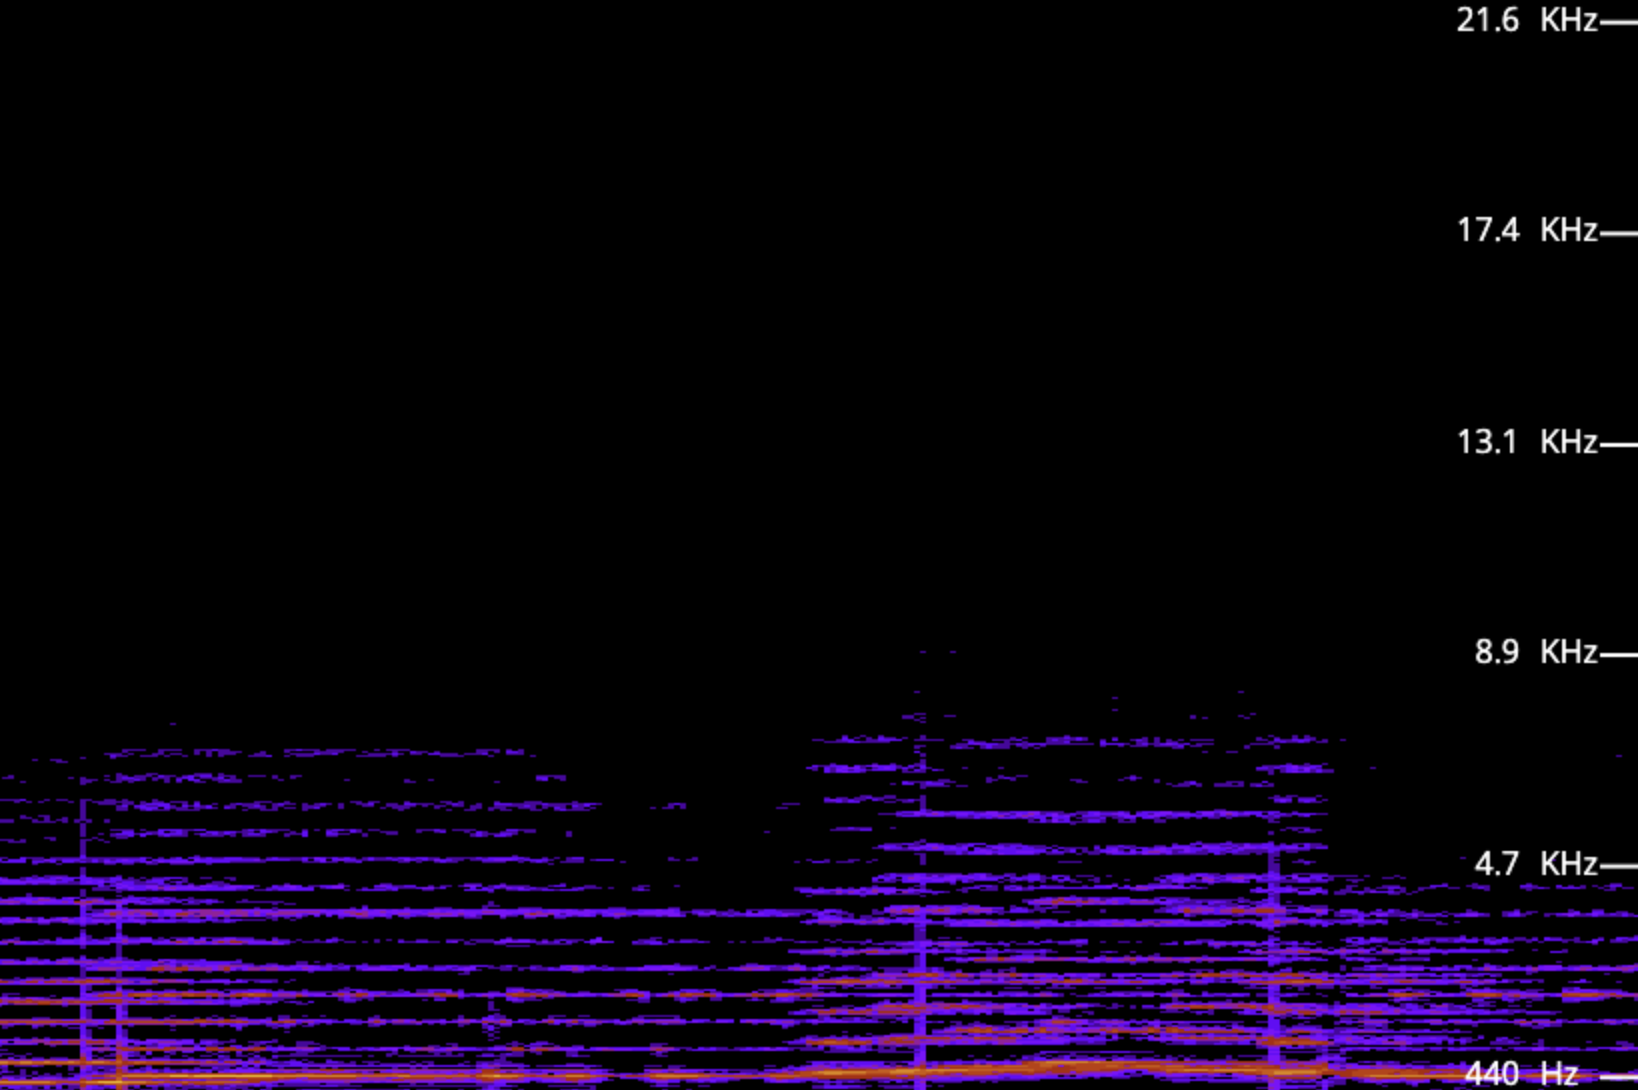
\includegraphics[width=\columnwidth]{figs/originalaudio.png}
\caption{Spectogram of Original audiosignal}
\end{figure}
\begin{figure}[ht]
    \centering  
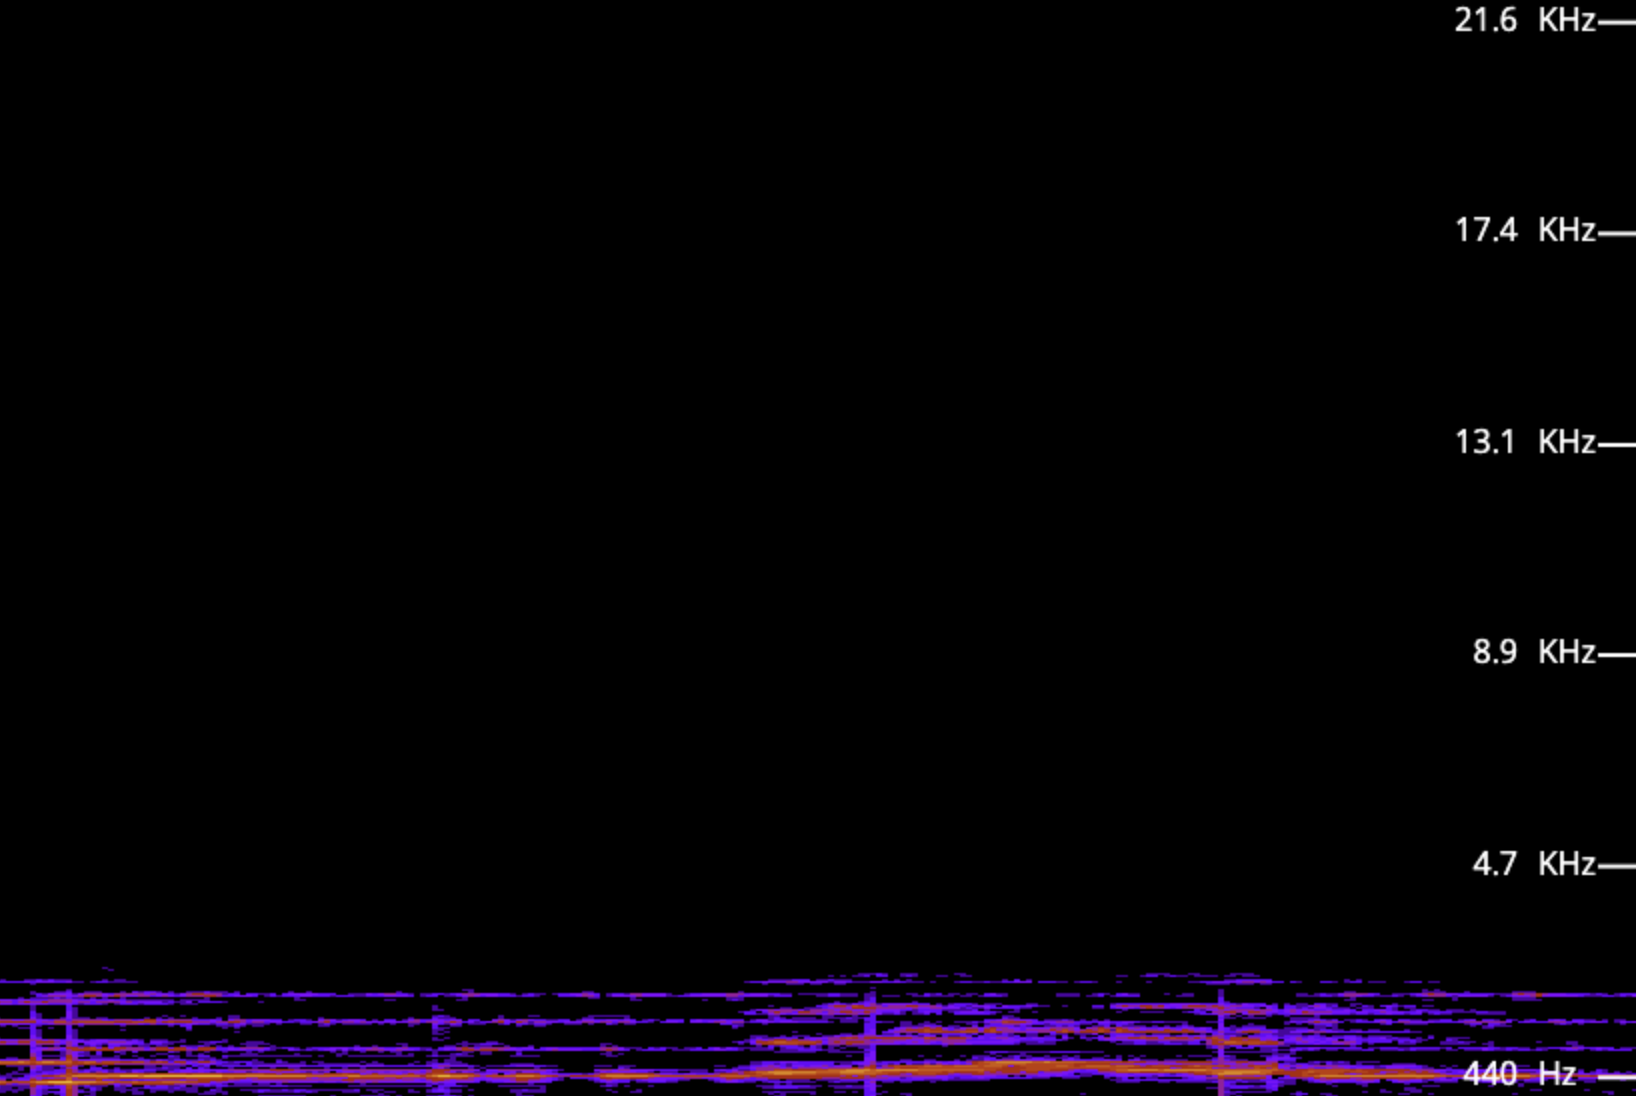
\includegraphics[width=\columnwidth]{figs/filteredaudio.png}
\caption{Spectogram after filtering audio signal}
\end{figure}
\begin{enumerate}[label=\thesection.\arabic*
,ref=\thesection.\theenumi]
\section{Difference equation}
\item Let
\begin{equation}
x(n) = \cbrak{\underset{\uparrow}{1},2,3,4,2,1} \label{prob:2.1}
\end{equation}
Sketch $x(n)$.\\ 
\item Let
\begin{multline}
y(n) + \frac{1}{2}y(n-1) = x(n) + x(n-2), 
\\
y(n) = 0, n < 0 \label{prob:2.2}
\end{multline}
Solve ans Sketch\\
\solution 
C code for generation of plots coordinates as text,\\
\begin{lstlisting}
https://github.com/Lohith12321/signals-and-systems/blob/main/audio_filtering/codes/plot1.c    
\end{lstlisting}
Python code for plotting the graph,\\
\begin{lstlisting}
https://github.com/Lohith12321/signals-and-systems/blob/main/audio_filtering/codes/plot1.py   
\end{lstlisting}
Plots for these text
\begin{figure}[ht]
    \centering  
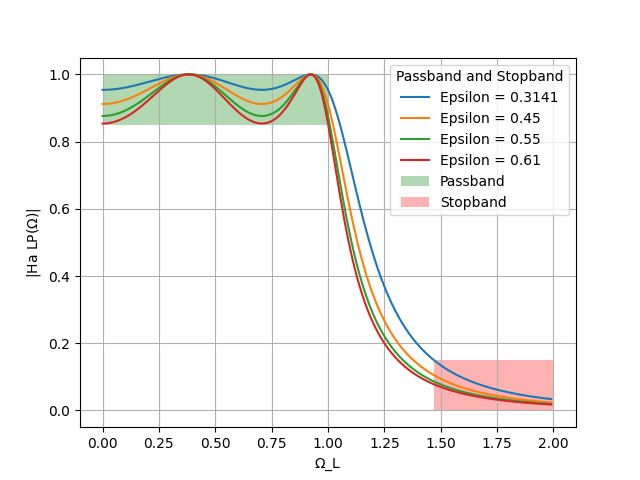
\includegraphics[width=\columnwidth]{figs/plot1.png}
\begin{center}
    \caption{Plot of x(n) and y(n)}
\end{center}
    \label{fig:plot1}
\end{figure}
\end{enumerate}
\begin{enumerate}[label=\thesection.\arabic*
,ref=\thesection.\theenumi]
\section{Z-Transform}
\item 
\begin{equation}
X(z)={\mathcal {Z}}\{x(n)\}=\sum _{n=-\infty }^{\infty }x(n)z^{-n}
\end{equation}
Show that
\begin{equation}
\label{eq:shift1}
{\mathcal {Z}}\{x(n-1)\} = z^{-1}X(z)
\end{equation}
and find
\begin{equation}
	{\mathcal {Z}}\{x(n-k)\} 
\end{equation}
\solution 
\begin{align}
    {\mathcal {Z}}\{x(n-1)\}&=\sum _{n=-\infty }^{\infty }x(n-1)z^{-n}\\
    {\mathcal {Z}}\{x(n-1)\}&=x(0)z^{0}+x(1)z^{-1}+...+\\
    {\mathcal {Z}}\{x(n-1)\}&=z^{-1}(x(0)z^{0}+x(1)z^{-1}...)\\
    {\mathcal {Z}}\{x(n-1)\}&=z^{-1}\sum _{n=-\infty }^{\infty }x(n)z^{-n}\\
    {\mathcal {Z}}\{x(n-1)\}&=z^{-1}X(z)
\end{align}
Similarly we can show that 
\begin{equation}
\label{eq:z_trans_shift}
	{\mathcal {Z}}\{x(n-k)\} = z^{-k}X(z)\\
\end{equation}
\item \begin{equation}
H(z) = \frac{Y(z)}{X(z)}
\end{equation}
from \eqref{prob:2.2} assuming that the $Z$-transform is a linear operation.
\\
\solution  Applying \eqref{eq:z_trans_shift} in \eqref{prob:2.2},
\begin{align}
Y(z) + \frac{1}{2}z^{-1}Y(z) &= X(z)+z^{-2}X(z)
\\
\implies \frac{Y(z)}{X(z)} &= \frac{1 + z^{-2}}{1 + \frac{1}{2}z^{-1}}
\label{eq:freq_resp}
\end{align}


\item Find the Z transform of 
\begin{equation}
\delta(n)
=
\begin{cases}
1 & n = 0
\\
0 & \text{otherwise}
\end{cases}
\end{equation}
and show that the $Z$-transform of
\begin{equation}
\label{eq:unit_step}
u(n)
=
\begin{cases}
1 & n \ge 0
\\
0 & \text{otherwise}
\end{cases}
\end{equation}
is
\begin{equation}
U(z) = \frac{1}{1-z^{-1}}, \quad \abs{z} > 1
\end{equation}


\solution It is easy to show that
\begin{equation}
\delta(n) \system{Z} 1
\end{equation}
and from \eqref{eq:unit_step},
\begin{align}
U(z) &= \sum _{n= 0}^{\infty}z^{-n}
\\
&=\frac{1}{1-z^{-1}}, \quad \abs{z} > 1
\end{align}
using the formula for the sum of an infinite geometric progression.
%
\item Show that 
\begin{equation}
\label{eq:anun}
a^nu(n) \system{Z} \frac{1}{1-az^{-1}} \quad \abs{z} > \abs{a}
\end{equation}
\solution 
\begin{align}
	a^nu(n) &\system{Z} \sum_{n = 0}^{\infty}\brak{a^nu\brak n}z^{-n} \\
        &\system{Z} \sum_{n = 0}^{\infty}\brak{a^n\brak{1}}z^{-n} \\
        &\system{Z} \sum_{n = 0}^{\infty}\brak{az^{-1}}^{n} \\
	&\system{Z} \frac{1}{1-az^{-1}} \quad \abs{z} > \abs{a}
\end{align}\\
\\

\item Let 
\begin{equation}
H\brak{e^{\j \omega}} = H\brak{z = e^{\j \omega}}.
\end{equation}
Plot $\abs{H\brak{e^{\j \omega}}}$.  Comment.  $H(e^{\j \omega})$ is
known as the {\em Discret Time Fourier Transform} (DTFT) of $x(n)$.\\
\solution 
Substituting $z = e^{j \omega}$ in \eqref{eq:freq_resp}, we get
\begin{align}
	\left|H\brak{e^{j\omega}}\right| &= \left|\frac{1 + e^{-2j\omega}}{1 + \frac{1}{2}e^{-j\omega}}\right| \\
									  &= \sqrt{\frac{\brak{1 + \cos{2\omega}}^2 + \brak{\sin{2\omega}}^2}{\brak{1 + \frac{1}{2}\cos{\omega}}^2 + \brak{\frac{1}{2}\sin{\omega}}^2}}\\
									  &= \frac{4|\cos{\omega}|}{\sqrt{5 + 4\cos{\omega}}}
\end{align}
\begin{align}
	\left|H\brak{e^{j\brak{\omega + 2\pi}}}\right| &= \frac{4|\cos\brak{\omega + 2\pi}|}{\sqrt{5 + 4\cos\brak{\omega + 2\pi}}} \\
											   &= \frac{4|\cos{\omega}|}{\sqrt{5 + 4\cos{\omega}}} \\
											   &= \left|H\brak{e^{j\omega}}\right|	
\end{align}
Therefore its fundamental period is $2\pi$ , which verifies that DTFT of a signal is always periodic.\\
The following code shows the plot
\begin{lstlisting}
    https://github.com/Lohith12321/signals-and-systems/blob/main/audio_filtering/codes/plot2.py
\end{lstlisting}
\begin{figure}[ht]
    \centering  
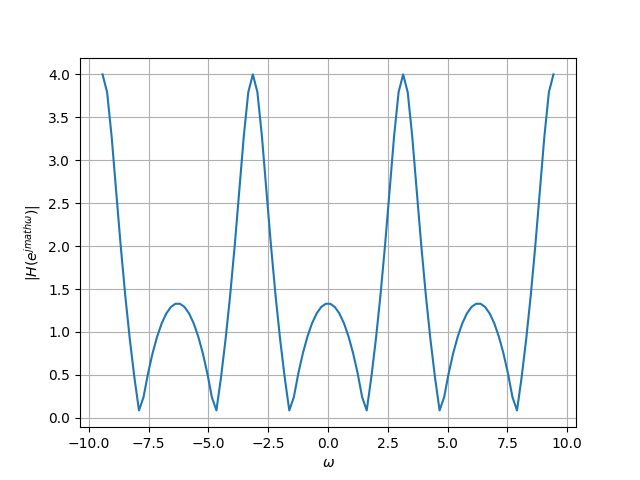
\includegraphics[width=\columnwidth]{figs/plot2.png}

\begin{center}
    \caption{$|H(e^{j\omega}|$}
\end{center}
    
    \label{fig:}
\end{figure}
\begin{enumerate}[label=\thesection.\arabic*
,ref=\thesection.\theenumi]
\section{Impulsive Response}
\item \label{prob:impulse_resp}
Find an expression for $h(n)$ using $H(z)$, given that 
%in Problem \ref{eq:ztransab} and \eqref{eq:anun}, given that
\begin{equation}
\label{eq:impulse_resp}
h(n) \system{Z} H(z)
\end{equation}
and there is a one to one relationship between $h(n)$ and $H(z)$. $h(n)$ is known as the {\em impulse response} of the
system defined by \eqref{prob:2.2}.
\\
\solution From \eqref{eq:freq_resp},
\begin{align}
H(z) &= \frac{1}{1 + \frac{1}{2}z^{-1}} + \frac{ z^{-2}}{1 + \frac{1}{2}z^{-1}}
\\
\implies h(n) &= \brak{-\frac{1}{2}}^{n}u(n) + \brak{-\frac{1}{2}}^{n-2}u(n-2)
\end{align}
using \eqref{eq:anun} and \eqref{eq:z_trans_shift}.
\item Sketch $h(n)$. Is it bounded? Convergent? \\
\solution The following code plots $h\brak{n}$ 
\begin{lstlisting}
    https://github.com/Lohith12321/signals-and-systems/blob/main/audio_filtering/codes/plot3.py
\end{lstlisting}
\begin{figure}[ht]
    \centering  
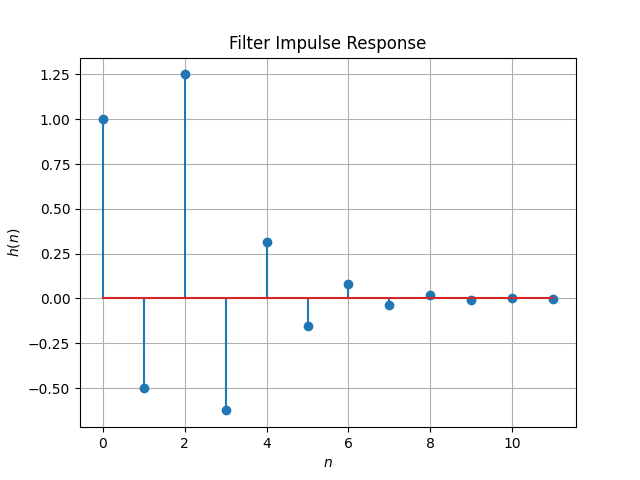
\includegraphics[width=\columnwidth]{figs/plot3.png}
\begin{center}
    \caption{$h(n)$}
\end{center}
    \label{fig:plot3}
\end{figure}
\item The system with $h(n)$ is defined to be stable if
\begin{equation}
\sum_{n=-\infty}^{\infty}h(n) < \infty \label{eq:stabilty_condn}
\end{equation}
Is the system defined by \eqref{prob:2.2} stable for the impulse response in \eqref{eq:impulse_resp}?\\
\solution For stable system \eqref{eq:stabilty_condn} should converge.\\
From ratio test
\begin{align}
    \lim_{n \to \infty}\left|\frac{h(n + 1)}{h(n)}\right|&<1 
\end{align}
As $n$ is very large,
\begin{align}
    u\brak{n}\approx \brak{n-2}\approx 1
\end{align}
\begin{align}
  \lim_{n \to \infty}  \brak{\frac{h(n + 1)}{h(n)}} = 1/2 <1
\end{align}
Therefore it converges and stable.
\item 
Compute and sketch $h(n)$ using 
\begin{equation}
\label{eq:iir_filter_h}
h(n) + \frac{1}{2}h(n-1) = \delta(n) + \delta(n-2), 
\end{equation}
%
This is the definition of $h(n)$.
\\
\solution\\
Definition of $h\brak{n}$: The output of the system when $\delta\brak{n}$ is given as input.\\

The following code plots Fig. \ref{fig:plot4}. Note that this is the same as Fig. 
\ref{fig:plot3}. 
\begin{lstlisting}
    https://github.com/Lohith12321/signals-and-systems/blob/main/audio_filtering/codes/plot4.py
\end{lstlisting}
\begin{figure}[ht]
    \centering  
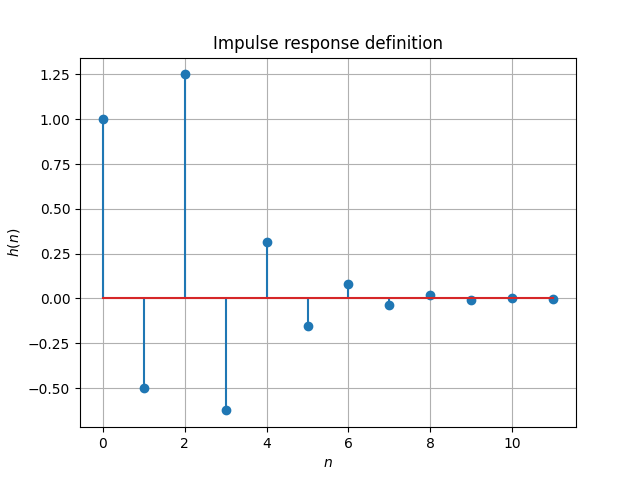
\includegraphics[width=\columnwidth]{figs/plot4.png}
\begin{center}
    \caption{$h(n)$}
\end{center}
    \label{fig:plot4}
\end{figure}


\item Compute 
%
\begin{equation}
\label{eq:convolution}
y(n) = x(n)*h(n) = \sum_{n=-\infty}^{\infty}x(k)h(n-k)
\end{equation}
%
Comment. The operation in \eqref{eq:convolution} is known as
convolution.
%
\\
\solution The following code plots Fig. \ref{fig:plot5}. Note that this is the same as 
$y(n)$ in  Fig. \ref{fig:plot1}. 
The following code gives above plot
\begin{lstlisting}
    https://github.com/Lohith12321/signals-and-systems/blob/main/audio_filtering/codes/plot5.py
\end{lstlisting}
\begin{figure}[ht]
    \centering  
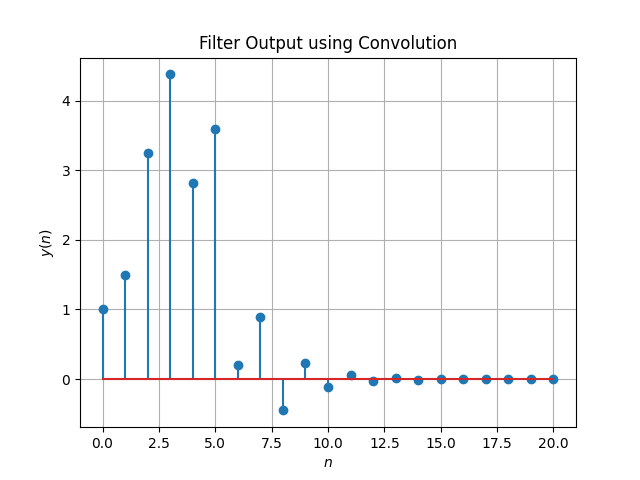
\includegraphics[width=\columnwidth]{figs/plot5.png}
\begin{center}
    \caption{$h(n)$}
\end{center}
    \label{fig:}
    \label{fig:plot5}
\end{figure}
\item Show that
\begin{equation}
y(n) =  \sum_{n=-\infty}^{\infty}x(n-k)h(k)
\end{equation}
\solution
In \eqref{eq:convolution}, we substitute $k = n - k$ to get
\begin{align}
y\brak{n} &= \sum_{k=-\infty}^{\infty}x\brak{k}h\brak{n - k} \\
		  &= \sum_{n - k=-\infty}^{\infty}x\brak{n - k}h\brak{k} \\
		  &= \sum_{k=-\infty}^{\infty}x\brak{n - k}h\brak{k}
\end{align}
\end{enumerate}
\begin{enumerate}[label=\thesection.\arabic*
,ref=\thesection.\theenumi]
\section{DFT and FFT}
\item
Compute
\begin{equation}
X(k) \define \sum _{n=0}^{N-1}x(n) e^{-\j2\pi kn/N}, \quad k = 0,1,\dots, N-1
\end{equation}
and $H(k)$ using $h(n)$.
\item Compute 
\begin{equation}
Y(k) = X(k)H(k)
\label{eq:fp}
\end{equation}
\item Compute
\begin{equation}
y\brak{n}={\frac {1}{N}}\sum _{k=0}^{N-1}Y\brak{k}\cdot e^{\j 2\pi kn/N},
\label{eq:inv-ft}
n = 0,1,\dots, N-1
\end{equation}
\solution The above three questions are solved using the code below\\
\begin{lstlisting}
    https://github.com/Lohith12321/signals-and-systems/blob/main/audio_filtering/codes/plot7.py    
\end{lstlisting}
This is the plot 
\item Repeat the previous exercise by computing $X(k), H(k)$ and $y(n)$ through FFT and IFFT.\\
\solution The solution of this question can be found in the code below.\\
\begin{lstlisting}
    https://github.com/Lohith12321/signals-and-systems/blob/main/audio_filtering/codes/plot6.py    
\end{lstlisting}
This code verifies the result by plotting the obtained result with the result obtained by IDFT.
\begin{figure}[ht]
    \centering  
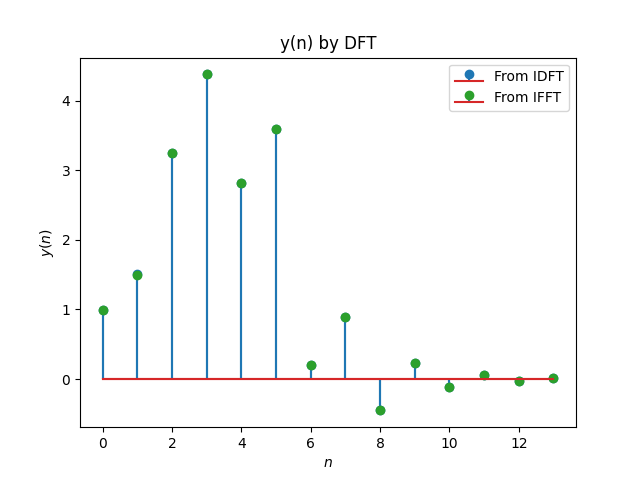
\includegraphics[width=\columnwidth]{figs/plot6.png}
\begin{center}
    \caption{$h(n)$}
\end{center}
\label{fig:plot4}
\end{figure}
\item Wherever possible, express all the above equations as matrix equations.\\
\solution The DFT matrix is defined as : 
\begin{align}
	\mtx{W} = 
	\begin{pmatrix}
		\omega^0 & \omega^0 & \ldots & \omega^0 \\
		\omega^0 & \omega^1 & \ldots & \omega^{N - 1} \\
		\vdots & \vdots & \ddots & \vdots \\
		\omega^0 & \omega^{N - 1} & \ldots & \omega^{(N -1)(N - 1)}
	\end{pmatrix}
\end{align}
where $\omega=e^{-\frac{j2\pi}{N}}$ . Now any DFT equation can be written as
\begin{align}
    \mtx{X} = \mtx{W}\mtx{x}
\end{align}
\noindent where
\begin{align}
	\mtx{x} = 
	\begin{pmatrix}
		x(0) \\ x(1) \\ \vdots \\ x(n - 1)
	\end{pmatrix}
\end{align}
\begin{align}
	\mtx{X} = 
	\begin{pmatrix}
		X(0) \\ X(1) \\ \vdots \\ X(n - 1)
	\end{pmatrix}
\end{align}
Thus we can rewrite  \eqref{eq:fp} as:
\begin{align}
	\mtx{Y} = \mtx{X}\odot\mtx{H} = \brak{\mtx{W}\mtx{x}}\odot\brak{\mtx{W}\mtx{h}}
\end{align}
where the $\odot$ represents the Hadamard product which performs element-wise multiplication.
\end{enumerate}

The below code computes $y\brak{n}$ by DFT Matrix and then plots it.\\
\begin{lstlisting}
    https://github.com/Lohith12321/signals-and-systems/blob/main/audio_filtering/codes/plot7.py
\end{lstlisting}
\begin{figure}[ht]
\centering
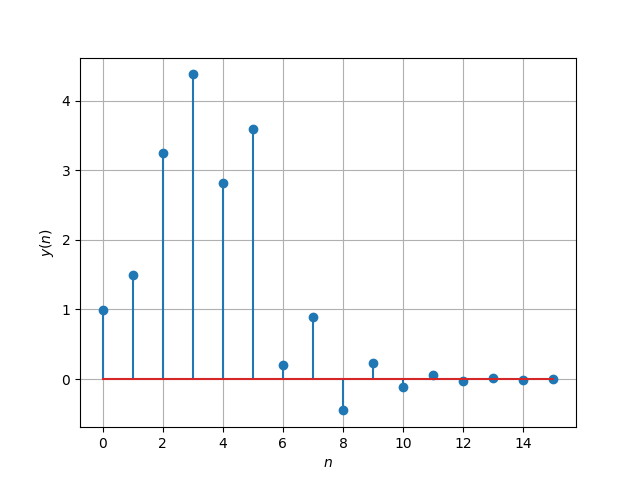
\includegraphics[width=\columnwidth]{figs/plot7.png}
\caption{$y(n)$ obtained from DFT Matrix}
\label{fig:plot6}
\end{figure}
\end{enumerate}
\begin{enumerate}[label=\thesection.\arabic*
,ref=\thesection.\theenumi]
\section{Exercises}
Answer the following questions by looking at the python code in Problem \ref{prob:audio_filter_problem}.
\item
\begin{lstlisting}
	output_signal = signal.lfilter(b, a, input_signal)
\end{lstlisting}
in Problem \ref{prob:audio_filter_problem} is executed through the following difference equation
\begin{equation}
\label{eq:iir_filter_gen}
 \sum _{m=0}^{M}a\brak{m}y\brak{n-m}=\sum _{k=0}^{N}b\brak{k}x\brak{n-k} 
\end{equation}
%
where the input signal is $x(n)$ and the output signal is $y(n)$ with initial values all 0. Replace
\textbf{signal. filtfilt} with your own routine and verify.\\

\solution The below code gives the output of an Audio Filter without using the built in function signal.lfilter.
\begin{lstlisting}
    https://github.com/Lohith12321/signals-and-systems/blob/main/audio_filtering/codes/plot8.py 
\end{lstlisting}

\begin{figure}[ht]
\centering
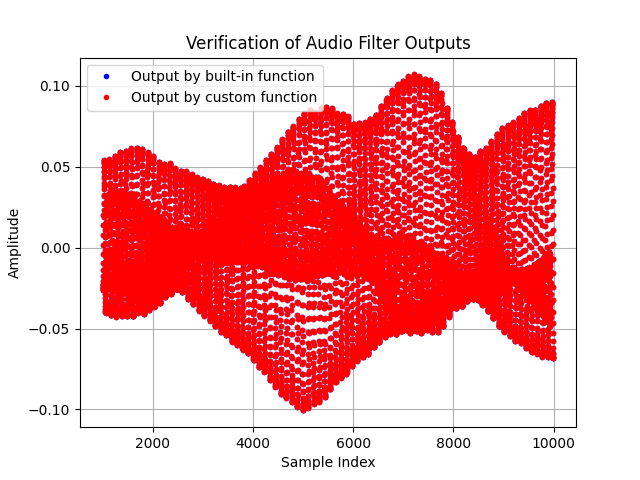
\includegraphics[width=\columnwidth]{figs/plot8.png}
\caption{Both the outputs using and without using function overlap}
\label{fig:plot8}
\end{figure}

\item Repeat all the exercises in the previous sections for the above $a$ and $b$.\\
\solution The code in \ref{prob:audio_filter_problem} generates the values of $a$ and $b$  which can be used to generate a difference equation.\\
And,
\begin{align}
    M &= 5\\
    N&=5
\end{align}
From \ref{eq:iir_filter_gen} 
\begin{align}
    &a\brak{0}y\brak{n} + a\brak{1}y\brak{n-1}+a\brak{2}y\brak{n-2}+a\brak{3}y\brak{n-3} \\ 
    &+ a\brak{4}y\brak{n-4} + a\brak{5}y\brak{n-5} + a\brak{6}y\brak{n-6} \\
    &=   b\brak{0}x\brak{n} + b\brak{1}x\brak{n-1}+b\brak{2}x\brak{n-2}+b\brak{3}x\brak{n-3} \\
    &+ b\brak{4}x\brak{n-4} + b\brak{5}x\brak{n-5} + b\brak{6}x\brak{n-6} 
\end{align}
Difference Equation is given by :
\begin{align}
	&y(n) - \brak{1}y(n - 1) + \brak{-4.89}y(n - 2) \nonumber \\
	&- \brak{-2.23}y(n - 3) + \brak{0.47}y(n - 4) \nonumber \\
	&= \brak{29.13\times 10^{-5}}x(n) + \brak{116.5\times 10^{-5}}x(n - 1) \nonumber \\
	&+ \brak{174.8 \times 10^{-5}}x(n - 2) + \brak{116.5 \times 10^{-5}}x(n - 3) \nonumber \\
	&+ \brak{29.1 \times 10^{-5}}x(n - 4)
\end{align}
From \eqref{eq:iir_filter_gen} 
\begin{align}
    H(z) &= \frac{b_0 + b_1 z^{-1} + b_2 z^{-2} + \ldots + b_M z^{-N}}{a_0 + a_1 z^{-1} + a_2 z^{-2} + \ldots + a_N z^{-M}}\\
    H(z) &= \frac{\sum_{k = 0}^{N}b(k)z^{-k}}{\sum_{k = 0}^{M}a(k)z^{-k}} \label{eq:trans-func}
\end{align}
Partial fraction on \eqref{eq:trans-func} can be generalised as:
\begin{align}
    H\brak{z}&= \sum_{i}\frac{r(i)}{1 - p(i)z^{-1}} + \sum_{j}k(j)z^{-j}
	\label{eq:trans-func-pfe}
\end{align}
Now,
\begin{align}
a^{n}u\brak{n} \system{Z} \frac{1}{1-az^{-1}} \label{eq:res-1}\\
    \delta\brak{n-k} \system{Z} z^{-k}\label{eq:res-2}
\end{align}
Taking inverse z transform of \eqref{eq:trans-func-pfe} by using \eqref{eq:res-1} and \eqref{eq:res-2}
\begin{align}
h(n) &= \sum_{i}r(i)[p(i)]^nu(n) + \sum_{j}k(j)\delta(n - j)
	\label{eq:h-n-expr}
\end{align}
The below code computes the values of $r\brak{i},p\brak{i} , k\brak{i}$ and plots $h\brak{n}$
\begin{lstlisting}
    https://github.com/Lohith12321/signals-and-systems/blob/main/audio_filtering/codes/plot12.py 
\end{lstlisting}
\renewcommand{\arraystretch}{2}
\begin{tabular}{|c|c|c|}
\hline 
\setlength{\tabcolsep}{1pt}
\textbf{Parameter}  &\textbf{Description} &\textbf{Formulae/Value} \\
\hline
$a\brak 0$ & First term of A.P & - \\
\hline
\textbf{$d$} & Commom difference & - \\
\hline
n & Count of terms starting from '0' & - \\
\hline
$a\brak n$ & $(n+1)^{th}$ term of the A.P & $a\brak0 + nd$ \\
\hline
$a\brak{21}$ & Value of $22^{nd}$ term & 149 \\

\hline
$S\brak n$ & Sum of (n+1) terms in A.P & $\left(\frac{n+1}{2}\right) (2a\brak0+nd)$ \\
\hline
\end{tabular}

\textbf{Stability of h(n)}:\\
According to \eqref{eq:stabilty_condn}
\begin{align}
H\brak{z} &= \sum_{n = 0}^{\infty} h\brak{n}z^{-n}\\
H(1)&= \sum_{n = 0}^{\infty}h(n)  = \frac{\sum_{k = 0}^{N}b(k)}{\sum_{k = 0}^{M}a(k)}< \infty
\end{align}
As both $a\brak{k}$ and $b\brak{k}$ are finite length sequences they converge.\\
The below code plots Filter frequency response
\begin{lstlisting}
    https://github.com/Lohith12321/signals-and-systems/blob/main/audio_filtering/codes/plot9.py
\end{lstlisting}
\begin{figure}[ht]
\centering
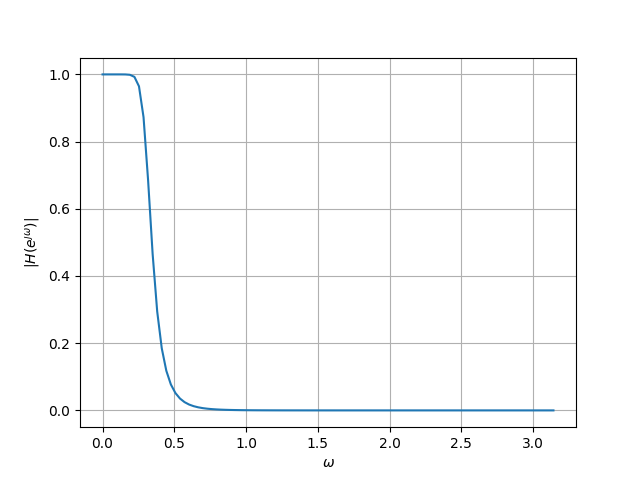
\includegraphics[width=1\columnwidth]{figs/plot9.png}
\caption{Frequency Response of Audio Filter}
\label{fig:plot9}
\end{figure}
The below code plots the Butterworth Filter in analog domain by using bilinear transform.
\begin{align}
    z=\frac{1+sT/2}{1-sT/2}
\end{align}
\begin{lstlisting}
    https://github.com/Lohith12321/signals-and-systems/blob/main/audio_filtering/codes/plot10.py
\end{lstlisting}
\begin{figure}[ht]
\centering
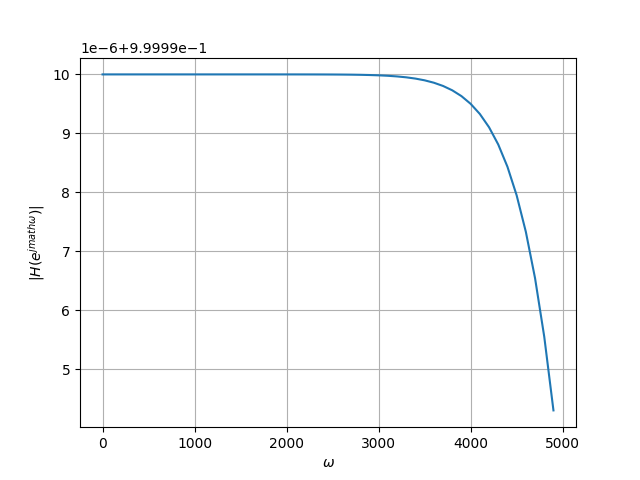
\includegraphics[width=1\columnwidth]{figs/plot10.png}
\caption{Frequency Response of Audio Filter}
\label{fig:plot10}
\end{figure}
The below code plots the Pole-Zero Plot of the frequency response.
\begin{lstlisting}
    https://github.com/Lohith12321/signals-and-systems/blob/main/audio_filtering/codes/plot11.py
\end{lstlisting}
\begin{figure}[ht]
\centering
\includegraphics[width=1\columnwidth]{figs/plot11.png}
\caption{As there are complex poles, so h(n) should be damped}
\end{figure}
\begin{figure}[ht]
\centering
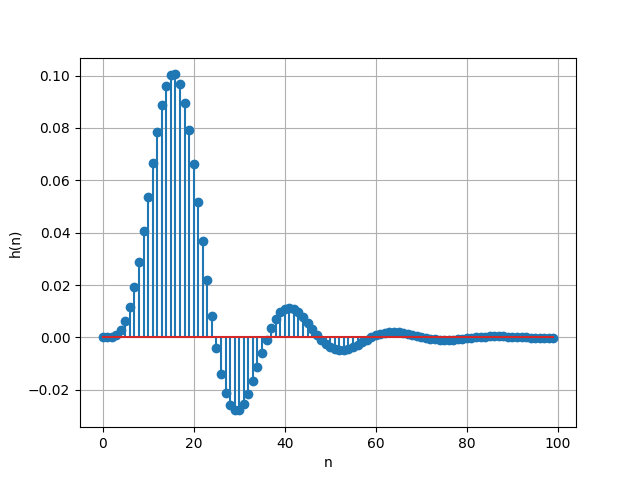
\includegraphics[width=1\columnwidth]{figs/plot12.png}
\caption{h(n) of Audio Filter.It is a damped sinusoid}
\label{fig:plot12}
\end{figure}
\item Implement your own fft routine in C and call this fft in python.\\

\solution The below C code computes FFT of a given sequence.
\begin{lstlisting}
    https://github.com/Lohith12321/signals-and-systems/blob/main/audio_filtering/codes/fft.c
\end{lstlisting}
The C function involved in computing the FFT is called in the below python code and the result is computed.\\

Before executing the python code. Execute the following command.
\begin{lstlisting}
    gcc −shared −o fft.so −fPIC fft.c
\end{lstlisting}
then execute this python code
\begin{lstlisting}
     https://github.com/Lohith12321/signals-and-systems/blob/main/audio_filtering/codes/fft.py
\end{lstlisting}
\item Find the time complexities of computing y(n)
using FFT/IFFT and convolution and Compare.\\
\solution The time required to compute y(n) using these two methods is calculated and the data is stored in a text file using the below C code.
\begin{lstlisting}
   https://github.com/Lohith12321/signals-and-systems/blob/main/audio_filtering/codes/plot13.c 
\end{lstlisting}
The below python code extracts the data from these text files and plots Time vs $n$ for comparison.
\begin{lstlisting}
    https://github.com/Lohith12321/signals-and-systems/blob/main/audio_filtering/codes/plot13.py
\end{lstlisting}
\begin{figure}[ht]
\centering
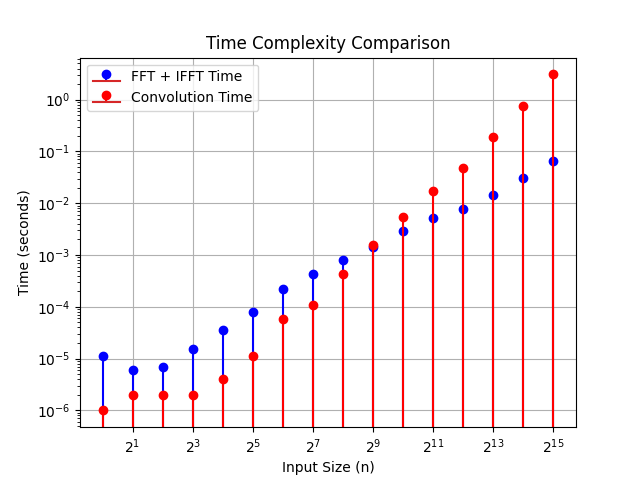
\includegraphics[width=1\columnwidth]{figs/plot13.png}
\caption{The Complexity of FFT+IFFT method is $ O(nlogn)$ where as by convolution is $O(n^2)$}
\label{fig:time_complexity}
\end{figure}
\item What is the sampling frequency of the input signal?\\
\solution The Sampling Frequency is 44.1KHz
\item
What is type, order and  cutoff-frequency of the above butterworth filter
\\
\solution The given butterworth filter is lowpass with order=6 and cutoff-frequency=2kHz.

\item
Modify the code with different input parameters and get the best possible output.

\solution
A better filtering was found on setting the order of the filter to be 5.
\end{enumerate}
\end{document}